\section{Semi-supervised learning}

Semi-supervised learning is a method of machine learning in which a small amount of labeled data is combined with a large amount of unlabeled data during training. 
Semi-supervised learning is intermediate between unsupervised (no labeled training data) and supervised learning (with only labeled training data). 
It is an example of weak supervision.

When combined with a small amount of labeled data, unlabeled data can significantly improve learning accuracy. 
Acquiring labeled data for a learning problem frequently necessitates the use of a skilled human agent (e.g., to transcribe an audio segment in \glsxtrshort{ASR} tasks).
The cost of labeling may thus make large, fully labeled training sets unfeasible, whereas acquiring unlabeled data is relatively inexpensive. Semi-supervised learning can be extremely useful in such situations.


\subsection{Wav2vec 2.0}

Due to self-supervised training, \glsxtrshort{Wav2vec 2.0} is one of the current \glsxtrshort{SOTA} models for \glsxtrshort{ASR}. 
This is a relatively novel concept in this sector. We can pre-train a model on unlabeled data, which is always more accessible, using this method of training. 
The model can then be fine-tuned for a specific purpose using a specific dataset.

The model consists of a multi-layer convolutional feature encoder $f: X \rightarrow Z$ that receives raw audio $X$ as input and produces \glsxtrshort{latent_speech_representations} ${z}_1,..., {z}_T$ for $T$ time steps. 
They are then supplied into a \glsxtrshort{Transformer} $g: Z \rightarrow C$, which generates representations ${c}_1,..., {c}_T$ that capture data from the full sequence. 
In the self-supervised objective, the output of the feature encoder is discretized to $q_t$ using a quantization module $Z \rightarrow Q$ to represent the objectives (Figure \ref{speech_representation_wav2vec2}). 
The approach constructs context representations over continuous speech representations, and self-attention captures dependencies throughout the whole sequence of latent representations.

\begin{figure}[hbtp]
    \centering
    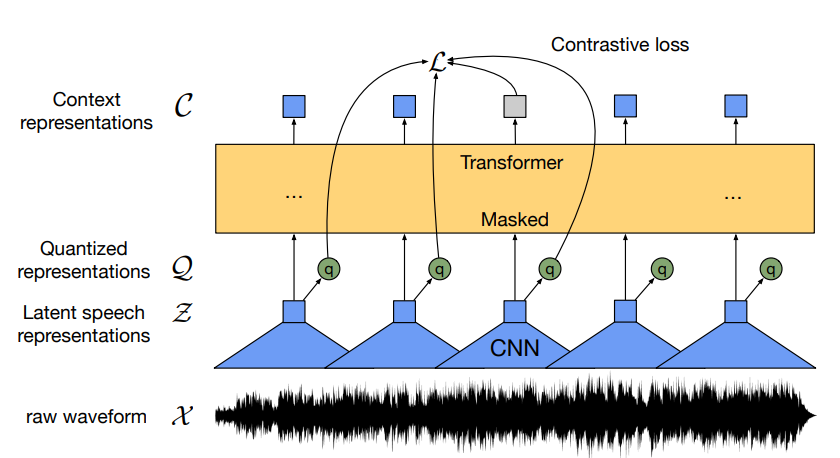
\includegraphics[width=0.8\textwidth]{figures/speech_representation_wav2vec2.PNG}
    \caption{Illustration of our framework which jointly learns contextualized speech representations and an inventory of discretized speech units.}
    \label{speech_representation_wav2vec2}
\end{figure}

\textbf{Feature encoder}: The encoder is made up of many blocks that include temporal convolution, layer normalization \cite{layer_normalization}, and the \glsxtrshort{GELU} activation function \cite{gelu}. 
The encoder's raw waveform input is normalized to zero mean and unit variance. 
The number of time-steps T that are input to the \glsxtrshort{Transformer} is determined by the encoder's total stride.

\textbf{Contextualized representations with Transformers}: The feature encoder's output is sent into a context network that uses the \glsxtrshort{Transformer} architecture \cite{Transformer}. 
We utilize a convolutional layer that acts as a relative positional embedding instead of fixed positional embeddings that encode absolute positional information. 
We implement layer normalization after adding the convolution output followed by a \glsxtrshort{GELU} to the inputs.

\textbf{Contrastive learning}: Contrastive learning is a notion that involves the input being altered in two ways. 
The model is then trained to recognize whether two input transformations are still the same item. 
The \glsxtrshort{Transformer} layers are the first method of transformation in \glsxtrshort{Wav2vec 2.0}; the second is quantization. 
In more technical terms, we would like to get such a context representation $c_t$ for a masked latent representation $z_t$ in order to guess the proper quantized representation $q_t$ among alternative quantized representations.

\begin{figure}[hbtp]
    \centering
    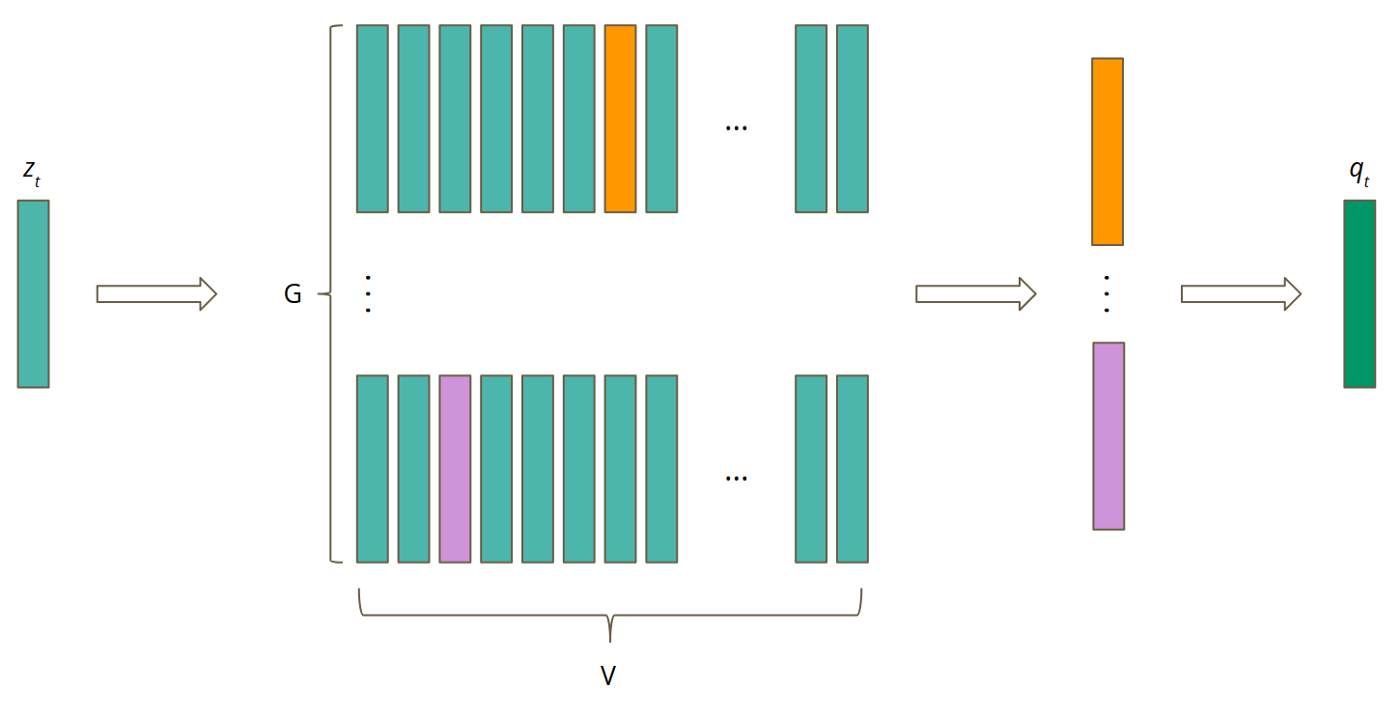
\includegraphics[width=0.8\textwidth]{figures/quantization_process.png}
    \caption{Quantization process: For each codebook, the best entry is extracted and concatenated with each other (from orange to purple entry)}
    \label{quantization_process}
\end{figure}

\textbf{Quantization module}: Quantization is a process of converting values from a continuous space into a finite set of values in a discrete space \cite{wav2vec2_towardsdatascience}. 
A language's number of phonemes is limited. 
Furthermore, the number of posible phoneme pairs is limited. 
It means that the same \glsxtrshort{latent_speech_representations} can correctly represent both of them. 
Furthermore, because the quantity is limited, we can design a codebook that contains all potential phoneme combinations. 
The quantization process then involves selecting the appropriate code word from the codebook. 
However,the total number of conceivable sounds is enormous. 
To make it easier to learn and use, we use product quantization \cite{product_quantization} to discretize the output of the feature encoder $z$ to a finite set of speech representations for self-supervised training. 
This choice yielded positive results, which acquired discrete units first and then contextualized representations. 
Concatenating quantized representations from several codebooks is what product quantization is all about. 
We take one item from each codebook and concatenate the resulting vectors $e_1,...,e_G$ (Figure \ref{quantization_process}), then perform a linear transformation $R^d \rightarrow R^f$ to get $q \in R^f$, given $G$ codebooks or groups with $V$ entries $e \in R^{V \times d/G}$. 


\subsection{Cross-lingual speech representation}

Cross-lingual learning seeks to create models that use data from other languages to improve performance.
By pretraining \glsxtrshort{Transformer} blocks with multilingual masked language models, unsupervised cross-lingual representation learning has shown great success \cite{lample2019cross, BERT}. 
The authors in \cite{xlsr53} studied cross-lingual speech representations by extending \glsxtrshort{Wav2vec 2.0} \cite{wav2vec2} to the cross-lingual setting. 
Their method teaches a single set of quantized latent speech representations that are shared by all languages.
They pre-trained \glsxtrshort{XLSR-53} on 56k hours of speech data from 53 languages (including Vietnamese language), then evaluated it on 5 languages from the BABEL benchmark (conversational telephone data) \cite{BABEL_dataset} and 10 languages from CommonVoice \cite{CommonVoice_dataset} - a corpus of read speech.

\begin{comment}
\textbf{Multilingual outperforms monolingual pretraining}: Pre-training on multiple languages results in
cross-lingual transfer and better speech representations.
Increasing the amount of pre-training data in multilingual pre-training setting is not the only reason for the increased accuracy, but on the same amount of pre-trained data, multilingual still outperforms monolingual pretraining. The authors believed that the similarity of the languages used in pretraining and fine-tuning is also meaningful.

\textbf{Cross-lingual representations transfer well to unseen languages}: On languages not seen during pre-training, multilingual pre-training still outperforms monolingual models pre-trained specifically on these languages. This implies that the learned representations capture generic features of the speech signal that are transferable across languages.

\textbf{Cross-lingual transfer learning improves low-resource language understanding}: Cross-lingual transfer and unsupervised cross-lingual representation learning are especially effective on low-resource languages. Empirical results have shown that, monolingual models perform badly on low-resource languages, but cross-lingual transfer is most effective in these cases.

\textbf{The transfer-interference trade-off: high vs. low-resource}: For languages with limited resources, because of positive transfer, multilingual models outperform monolingual models; however, multilingual models perform worse on high-resource languages. However, by increasing model capacity, the gap between multilingual and monolingual models for high-resource languages can be narrowed.

\textbf{Multilingual fine-tuning}: Multilingual fine-tuning outperforms monolingual fine-tuning and allows us to use a single model for multiple languages.


\subsection{Domain-shift in self-supervised pre-training}

Self-supervised learning of speech representations has been a very interesting research topic, but most work has been dedicated to a single domain, such as read audio books, for which large amounts of labeled and unlabeled data exist. 
In \cite{robust_wav2vec2}, the authors looked at more general scenarios in which the domain of the unlabeled data for pre-training differs from the domain of the labeled data for fine-tuning, which may differ from the domain of the test data.

\textbf{Adding pre-training data}: Adding in-domain pre-training data always helps to improve the performance, while adding out-of-domain pre-training data is not always helpful. Performance is further enhanced for both joint training and continual training when there is more in-domain unlabeled data.

\textbf{Pre-training on diverse data}: It demonstrates that pre-training on three domains yields better results than pre-training on two domains, which yields better results than pre-training on one domain, no matter what labeled data is used.

\textbf{Effect of pre-training data similarity to target domain}: If the unlabeled data, labeled data, and target domain all have a perfect domain match, then more unlabeled data consistently enhances the performance.

\end{comment}

\subsection{In-domain Match Level and Diversity Level}

In this part, to better and easier analyze the effect of pre-training data on the performance of cross-lingual and domain-shift experiments, we introduce 2 new concepts, namely \textbf{"In-domain Match Level"} and \textbf{"Diversity Level"}. 

\textbf{In-domain Match Level}: Given 3 datasets A, B and C, where A is the target telephone dataset used for recognition, B is also recorded by the telephone but its conversation is different from A's and C is the audio book recordings. 
The dataset B is more overlapped with the A than the C because both A and B are telephone recordings, so the \textbf{In-domain Match Level} of B is higher than the one of C. 
In general, the \textbf{In-domain Match Level} is determined by the similarity between recording conditions, naturalness and conversational topics.

\textbf{"Diversity Level"}: Given another dataset D, which is recorded by more speakers with more diverse accents than B and C, then the \textbf{Diversity Level} of D is the highest compared to the rest. 
To some extent, the \textbf{Diversity Level} of the multilingual dataset is higher than the monolingual one because the first is able to represent more learnable phonemes which are likely to be helpful to target language in semi-supervised learning.
